\documentclass[conference]{IEEEtran}
% IEEE camera-ready asks for Acrobat 5.0 compatibility, which is PDF 1.4.
\pdfminorversion=4
\IEEEoverridecommandlockouts

\usepackage{cite}
\usepackage{amsmath,amssymb,amsfonts,amsthm}
\usepackage{graphicx}
\usepackage{booktabs}
\usepackage{textcomp}
\usepackage{url}

\pdfinfo{
  /Title (Herd Immunity and Learning Externalities in Markets of Shared Foundation Models)
  /Author (Vignesh Nagarajan, Shriraghav Ashok)
}

\newtheorem{theorem}{Theorem}
\newtheorem{lemma}{Lemma}
\newtheorem{proposition}{Proposition}
\newtheorem{corollary}{Corollary}
\theoremstyle{definition}
\newtheorem{remark}{Remark}

\newcommand{\Neff}{N_{\mathrm{eff}}}
\newcommand{\lmax}{\lambda_{\max}}
\newcommand{\ones}{\mathbf{1}\mathbf{1}^{\top}}
\newcommand{\gPO}{\gamma_{\mathrm{PO}}}
\newcommand{\seff}{s_{\mathrm{eff}}}
\newcommand{\vecop}{\operatorname{vec}}

\begin{document}

\title{Herd Immunity and Learning Externalities in Markets of Shared Foundation Models}

\author{\IEEEauthorblockN{Vignesh Nagarajan\textsuperscript{\dag}}
\IEEEauthorblockA{Texas A\&M University\\
College Station, TX, USA\\
vigneshn26@tamu.edu}
\and
\IEEEauthorblockN{Shriraghav Ashok\textsuperscript{\dag}}
\IEEEauthorblockA{University of California, Berkeley\\
Berkeley, CA, USA\\
sashok24@berkeley.edu}
\thanks{\textsuperscript{\dag}These authors contributed equally to this work.}}

% The BigData 2026 camera-ready instructions ask for no page 1 copyright line
% and give no ISBN. If the chairs send the exact string, put it here and
% uncomment both this line and the \IEEEpubidadjcol below.
% \IEEEpubid{979-8-XXXX-XXXX-X/26/\$31.00~\copyright2026 IEEE}

\maketitle

\begin{abstract}
Every firm that prices, lends or ranks with machine learning wants its model
current, so it retrains on the newest data. However, that data was produced in
part by its own model and by every competitor's. When many firms fine-tune the
same foundation model, one firm's retraining changes what every other firm
learns from next, and no firm accounts for it. This paper models that market
and shows it is stable exactly when one number, the feedback reproduction
number, stays below one. That number depends on how many independent models
sit under the market, not on how many firms there are. When firms draw on a
common pool, fifty firms built on one vendor's model behave like one learner
with fifty times the footprint. On this foundation we
derive three remedies. Retraining in smaller steps helps only below a critical
crowding level. Correcting for feedback works like vaccination, and the share
of firms that must correct follows the epidemiological coverage formula for an
imperfect vaccine, including an efficacy below which no coverage is enough. A
tax on aggressive adaptation closes the gap between private and social
incentives, and without it every market of two or more firms over-adapts. We
confirm the base law in one measured check, which reruns an order-flow market
simulator and reproduces its published amplification to every reported digit.
Every other check of the theory confirms a formula against the model it came
from, and is labeled that way. A pilot on 79 deployed language models puts the shared
fraction near 0.43 on an error-correlation proxy. Ultimately, the framework gives a supervisor one
market-level quantity and three instruments that act on it.
\end{abstract}

\begin{IEEEkeywords}
algorithmic monoculture, foundation models, herd immunity, learning
externalities, performative prediction, Pigouvian taxation, systemic risk
\end{IEEEkeywords}

\section{Introduction}

\subsection{Problem definition}
The stability of a market in which firms price, lend and rank with machine
learning is driven by the mechanics of retraining. Consider fifty dealers
quoting the same bonds. Each dealer retrains its pricing model on the order
flow it saw since the last retraining, and each one, tested on its own, is
sound: replayed against its own history, it settles down. Placed in one
market, the fifty can still diverge. The flow a dealer sees depends on how the
other forty-nine priced, so every retraining changes what every other dealer
learns from next, and none of the fifty models accounts for that. We term this
a \emph{learning externality}. The problem grows more acute as firms
increasingly learn from the same place: firms that fine-tune one vendor's
foundation model make correlated errors \cite{kim2025}. Models are validated
one at a time, and a common assumption behind that practice is that a market
of individually stable models is itself stable.

% \IEEEpubidadjcol
\subsection{Current approaches}
Looking at the existing literature, the idea that sensible individual behavior
can add up to collective fragility is well established. Banks that each
diversify optimally end up holding the same portfolios and fail together
\cite{beale2011,wagner2010}. Quantitative funds running similar strategies
unwound together in August 2007, and no single fund's risk report showed the
crowding \cite{khandani2007}. However, these accounts describe agents that
hold positions, not agents that learn.

The tool used today for learning systems, meanwhile, examines one model at a
time: a learner whose deployment reshapes its own data converges under
repeated retraining when its performative modulus $m$ stays below one
\cite{perdomo2020}. In a market that certificate is not enough, because none
of these approaches separates the stability of a model from the stability of
the market it is deployed in.

This blind spot is particularly consequential now, since the agents not only
learn but increasingly learn from a shared foundation model. As this paper
shows, such firms push the market in correlated directions, and it is this
correlation, rather than the number of firms, that decides whether the market
is stable. A supervisor is therefore left without a market-level quantity to
measure.

\subsection{Proposed approach}
To address these limitations, this paper proposes a four-part framework.
First, we define a market-level quantity, the \emph{feedback reproduction
number} $m_N$, the factor by which a shared disturbance grows per round of
retraining. We show that it is governed by $m_N = \Neff m_1$, where the
\emph{effective crowding} $\Neff$ depends on the leading eigenvalue of a
correlation matrix of the firms' response directions (Section~\ref{sec:crowd}).
Second, we derive an exact stability threshold for a market mixing corrected
and uncorrected firms, and show that correction and model diversity substitute
for each other along a frontier we compute (Section~\ref{sec:herd}). Third, we
analyze two further instruments, retraining in smaller steps and a Pigouvian
fee that prices the externality (Section~\ref{sec:levers}). Fourth, we check
every closed form numerically and label each check by the kind of evidence it
provides (Section~\ref{sec:results}). Full proofs, code and 542 numerical
certificates are public \cite{price2026}.

\subsection{Results overview}
The framework yields one stability condition and three instruments that act on
it. The market converges exactly when $m_N < 1$, and $m_N$ depends on how many
independent models sit under the market. In a common-pool market at full
spillover (Section~\ref{sec:baseline}), fifty firms built on one vendor's
model behave like one learner fifty times larger, while fifty firms whose
models push the market in unrelated directions behave like one firm. Diversity
indices built on mean similarity can call an unstable market safe.

The herd-immunity threshold reduces to the coverage a population needs when a
vaccine is imperfect \cite{anderson1985,fine2011}, together with an efficacy
below which no coverage is enough. The clean threshold obtained by assuming
perfect correction is not safe to use on its own. Checked against the exact
spectral radius on random markets, it is wrong in the dangerous direction,
calling $11.8\%$ of configurations stable that are unstable at every finite
correction strength. We therefore state the exact threshold as the theorem and
keep the clean limit as a corollary with its error direction stated.
Additionally, retraining in smaller steps helps only below a critical crowding
level, and without the fee every market of two or more firms adapts too
aggressively.

These results reveal that the provenance of the models, rather than the number
of firms, is what makes a market stable or unstable. The scope of the claim is
deliberately narrow. This paper is not an empirical study of a deployed
market. One numerical check is measured, in an order-flow simulator we built
for earlier work \cite{reflex2026}, and the rest confirm the formulas against
the model they came from. A pilot estimate of the key eigenvalue on a proxy,
error correlations across 79 deployed language models, is in
Section~\ref{sec:pilot}. It has not been measured in a deployed market.

\section{Background}

\subsection{Collective behavior}
This paper builds upon the study of collective behavior. Threshold models
explain how a behavior spreads once enough others have adopted it
\cite{granovetter1978}, and informational cascades explain why people
rationally copy their predecessors and why the resulting consensus is fragile
\cite{bikhchandani1992}. Both describe people imitating people. In our setting
nobody imitates anyone: firms become correlated because they learn from shared
data through shared models. The epidemiological link is consequently an
identity rather than an analogy. The reproduction number $R_0$ is defined as
the spectral radius of a next-generation operator \cite{diekmann1990}, $m_N$
is the spectral radius of a linearized retraining operator, and so the two
thresholds are the same statement. This is why the vaccination results carry
over with their refinements, including the imperfect-vaccine law. Contact
structure matters as well: on scale-free networks the epidemic threshold
vanishes altogether \cite{pastor2001}. In this study the alignment matrix
plays the role of the contact structure.

\subsection{Algorithmic monoculture}
When many firms adopt one algorithm, welfare can fall even if that algorithm
is the better one, because independent errors stop cancelling
\cite{kleinberg2021}. Shared models also concentrate harm on the same
individuals \cite{bommasani2022}, and a shared evaluation algorithm changes
outcomes in matching markets \cite{peng2024}. However, these results describe
a market at rest. None gives a stability boundary, so a market can look sound
at equilibrium and still be one retraining away from diverging.

\subsection{Performative prediction}
Performative prediction studies learners whose deployments shift their own
data \cite{perdomo2020}. With several learners in one environment, convergence
conditions exist that bound scalar sensitivities against curvature
\cite{narang2023}, and in the fully aligned case, increasing learning rates
and agent counts can drive the dynamics into chaos \cite{piliouras2023}. By
contrast, our condition bounds a spectral radius, and
Proposition~\ref{prop:scalars} exhibits two markets that agree on every scalar
such a criterion reads but differ in stability. This paper additionally
composes two single-learner tools with the market: lazy deployment, in which a
learner takes a few gradient steps per round \cite{mendler2020}, and
feedback-aware updates that correct for the learner's own influence
\cite{izzo2021,miller2021}.

\subsection{Systemic risk}
Reading the largest eigenvalue of a correlation matrix as the weight of a
common market mode is standard in econophysics \cite{laloux1999,plerou2002}.
We compute it from a different matrix, response directions instead of returns,
and it enters a stability condition rather than a portfolio.

\section{A Market of Retraining Firms}

\subsection{Baseline model}\label{sec:baseline}
We begin with $N$ dealers quoting the same instruments. Dealer $i$ deploys a
pricing model with parameters $h_i \in \mathbb{R}^d$. Each round it retrains
by minimizing its expected loss on the order flow it has seen since the last
round,
\begin{equation}
  h_i^{t+1} = \arg\min_{h}\;
  \mathbb{E}_{z \sim \mathcal{D}_i(h_1^{t},\dots,h_N^{t})}\,\ell(z;h).
  \label{eq:rrm}
\end{equation}
This is repeated risk minimization \cite{perdomo2020} with one change: the
flow distribution $\mathcal{D}_i$ depends on every dealer's deployed model,
not only on dealer $i$'s. Three constants describe the loop near equilibrium,
and they are the constants of \cite{perdomo2020}. The response strength
$\varepsilon$ is the sensitivity of $\mathcal{D}_i$ to dealer $i$'s own
deployment: how far its flow moves per unit change in its quotes. The
sensitivity $\beta$ is the Lipschitz constant of the loss gradient in the
data: how far the dealer's optimum moves per unit shift in the flow. The
curvature $\gamma$ is the strong-convexity constant of the loss in $h$. A
dealer retraining alone converges when its performative modulus
$m_1 = \varepsilon\beta/\gamma$ is below one \cite{perdomo2020}. In the linear-quadratic model that (A1) below
linearizes to, the slope of its retraining map is exactly $-m_1$, so the
condition is also necessary.

Dealers are coupled through one pool of informed order flow. A change in
dealer $j$'s quotes shifts the flow dealer $i$ trains on by
$\kappa \in [0,1]$ times the shift it causes in dealer $j$'s own flow.
Stacking the $N$ retraining maps and differentiating at the joint equilibrium
gives the Jacobian $J = -m_1[(1-\kappa)I + \kappa\ones]$. Each diagonal entry,
$-m_1$, is a dealer's own loop. Each off-diagonal entry, $-\kappa m_1$, is the
effect of one competitor's deployment on that dealer's next model. The largest
mode, the one in which all dealers move together, has size
$m_1(1+\kappa(N-1))$. The market therefore goes unstable at a response
strength $1+\kappa(N-1)$ times smaller than any single dealer can tolerate.
This law comes from our earlier work \cite{reflex2026}, and
Section~\ref{sec:results} measures it. Everything that follows replaces one
object in it: the all-ones matrix $\ones$, which states that every dealer
pushes the flow in the same direction.

\emph{What $\kappa$ measures.} The spillover $\kappa$ is a ratio: the shift a
competitor's deployment causes in the flow a dealer trains on, relative to the
shift the dealer's own deployment causes. Whether it depends on $N$ is a
property of the market, and two cases bracket it. In a \emph{common-pool}
market every firm trains on a sample of one shared state, here the toxicity of
the informed pool. An informed trader can trade against every dealer whose
quote is stale, so when one dealer tightens, the informed share of the flow
rises at every dealer. Composition is not divided among those who observe it,
so $\kappa$ does not shrink as dealers are added. This is the market the
simulator of \cite{reflex2026} implements and the one this paper analyzes. In
a \emph{diversion} market a firm's repricing only displaces a fixed volume of
orders onto its competitors. Total flow is conserved, each competitor receives
a $1/(N-1)$ share, and $\kappa = \kappa_d/(N-1)$. In general
\begin{equation}
  \kappa = \kappa_c + \frac{\kappa_d}{N-1},
  \label{eq:kappa}
\end{equation}
with a common-pool part $\kappa_c$ and a diversion part $\kappa_d$.

The defining feature of this setting is economic. A price change is a transfer
between parties. Changing the data a competitor learns from, by contrast,
changes its forecasting technology, which is a real efficiency loss and a
technological externality in the classical sense \cite{buchanan1962}.
Moreover, nothing in dealer A's validation data contains dealer B, so no
single-model test can detect it.

\subsection{Alignment matrix}
In a real market firms do not all push the same way. We therefore give firm
$i$ a response Jacobian $E_i \in \mathbb{R}^{d\times d}$, describing how its
deployment reshapes the flow it faces. The alignment matrix $R$ has entries
\begin{equation}
  r_{ij} = \frac{\langle \vecop E_i, \vecop E_j \rangle}
                {\|E_i\|_F\,\|E_j\|_F},
  \label{eq:align}
\end{equation}
the correlation between two firms' feedback directions. It is positive
semidefinite with ones on the diagonal, like a correlation matrix of returns,
but it measures something different: whether two firms' models distort the
market the same way.

The analysis rests on four standing assumptions. (A1) Stability statements
linearize the joint map at equilibrium, and the simulator serves as the
nonlinear check. (A2) Firms have equal moduli $m_i = m_1$; unequal moduli give
two-sided bounds. (A3) Firms retrain on a common clock. (A4) Firms couple
through one pool with scalar spillover $\kappa$.

\begin{lemma}[Reduction]\label{lem:reduction}
Suppose each firm's deviation from equilibrium is a scalar $x_i$ along its own
unit response direction, and all $\|E_i\|_F$ equal $\varepsilon$. Each firm
feels its own distortion in full and a competitor's with weight $\kappa$, both
measured along its own direction. Each firm best-responds under a
$\gamma$-strongly convex objective with sensitivity $\beta$. Then the joint
retraining map is linear with Jacobian
\begin{equation}
  J = -m_1\bigl[(1-\kappa)I + \kappa R\bigr].
  \label{eq:jac}
\end{equation}
\end{lemma}

The proof takes two lines. The pool carries the total distortion
$\sum_j x_j E_j$, firm $i$ reads it along its own direction, and the inner
products are $\varepsilon r_{ij}$. The hypothesis that firms read the pool
only along their own direction is literal in a dealer market, because a dealer
sees order flow only where it quotes. Flow that a competitor's repricing
pushes into instruments the dealer does not trade never reaches its training
set, however large that set is. This is why two firms perturbing the market in
orthogonal directions do not affect each other, and why $R$ appears at all.

The lemma uses $E_i$ only through its norm $\varepsilon$ and the inner
products $r_{ij}$, and it uses the objective only through its curvature
$\gamma$ along the firm's own response direction and its sensitivity $\beta$
to the distortion the firm feels, $f_i$. For a smooth strongly convex loss
these are second derivatives at equilibrium: locally
$\ell_i \approx \tfrac{\gamma}{2}x_i^2 + \beta f_i x_i$, and the best response
is $x_i^{+} = -(\beta/\gamma) f_i$. Strong convexity \cite{perdomo2020} is
therefore needed along one direction per firm, not on all of
$\mathbb{R}^{d\times d}$, and (A1) is what licenses the quadratic form.

\begin{figure*}[t]
  \centering
  \begin{minipage}[t]{0.32\textwidth}
    \centering
    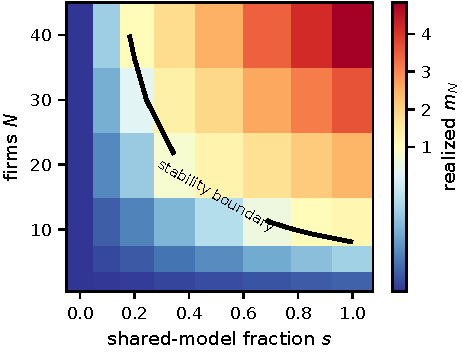
\includegraphics[width=\linewidth]{figures/fig_phase.pdf}
    \caption{Dry run in the reference environment: $m_N$ across 48 cells of firm
  count $N$ and shared-model fraction $s$, with the predicted stability
  boundary. It agrees with Theorem~\ref{thm:align} in every cell to within
  $7.1\times10^{-15}$ (Section~\ref{sec:results}).}
    \label{fig:phase}
  \end{minipage}\hfill
  \begin{minipage}[t]{0.32\textwidth}
    \centering
    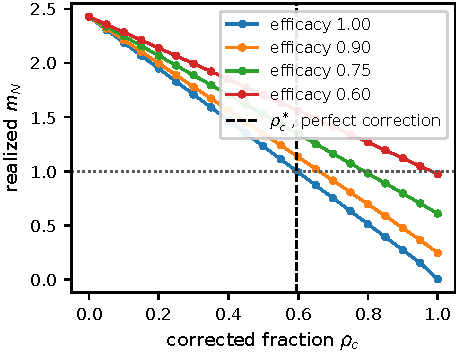
\includegraphics[width=\linewidth]{figures/fig_herd.pdf}
    \caption{Dry run: market modulus $m_N$ against corrected fraction at
  $N = 20$, $m_1 = 0.15$, $\kappa = 0.8$, $s = 1$, for four efficacies. The
  dashed line is the perfect-correction threshold. The gap between it and each
  crossing is the error Section~\ref{sec:herd} describes, not noise.}
    \label{fig:herd}
  \end{minipage}\hfill
  \begin{minipage}[t]{0.32\textwidth}
    \centering
    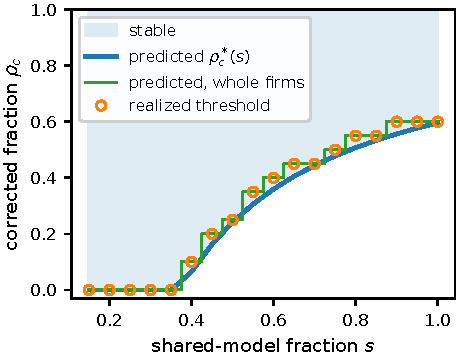
\includegraphics[width=\linewidth]{figures/fig_substitution.pdf}
    \caption{Dry run: the corrected fraction needed for stability against
  shared-model fraction $s$, at $N = 20$, $m_1 = 0.15$, $\kappa = 0.8$ and
  near-perfect correction. Predicted and realized thresholds agree in whole
  firms at 18 of 18 points. Everything above the curve is stable.}
    \label{fig:subst}
  \end{minipage}
\end{figure*}

\emph{Beyond dealers.} How far the own-direction hypothesis carries depends on
what a firm can observe. In lending it holds through selective labels: a
lender observes repayment only for applicants it approves, so it reads a shift
in the borrower population only along the features it lends on. In ranking it is an approximation: a platform logs
feedback only on what it shows, but its logs can record shifts in user
behavior that it did not cause and does not act on. Where the hypothesis
fails, the state no longer reduces to one scalar per firm and $\Neff$ is no
longer given exactly by Theorem~\ref{thm:align}; we do not analyze that case.
The coupling differs by domain as well. Borrowers who adapt a feature to many
lenders' models form a common pool. Applicants rejected by one lender who
apply to the next are diversion. Both are present in a real credit market.

\section{Effective Crowding}\label{sec:crowd}
Because firms that push in unrelated directions do not interact, counting
firms gives the wrong answer. The right count is the leading eigenvalue
$\lmax(R)$, which runs from $1$, when all response directions are orthogonal,
to $N$, when they all coincide.

\begin{theorem}[Alignment sets the reproduction number]\label{thm:align}
Under (A1)--(A4) and Lemma~\ref{lem:reduction}, the market's spectral radius
is
\begin{equation}
  m_N = \Neff\, m_1, \qquad
  \Neff = 1 + \kappa\bigl(\lmax(R) - 1\bigr),
  \label{eq:mn}
\end{equation}
and the market is stable if and only if $m_N < 1$.
\end{theorem}

Put plainly, a market behaves like $\Neff$ copies of one firm, and $\Neff$
counts independent models, not firms.

Three cases make the theorem concrete. First, if every firm shares one model,
$R = \ones$ and we recover the symmetric law $\Neff = 1 + \kappa(N-1)$.
Second, if every firm's direction is orthogonal to every other, $R = I$ and
$\Neff = 1$: a hundred firms pushing in a hundred unrelated directions are
dynamically one firm. Third, if each firm's response is a share $s$ from a
common foundation model, vendor or pretraining corpus and $1-s$ its own,
alignments concentrate at $s$ and $\Neff \to 1 + \kappa s(N-1)$. One bound
holds throughout: $\Neff \ge 1$, so interaction never makes a market more
stable than its members are alone.

\begin{remark}[Conserved flow]\label{rem:conserved}
Theorem~\ref{thm:align} holds for any $\kappa$. With \eqref{eq:kappa} and
supply-chain alignment,
\begin{equation}
  \Neff = 1 + \kappa_d\,s + \kappa_c\,s\,(N-1).
  \label{eq:neffsplit}
\end{equation}
Crowding grows with the number of firms only through the common-pool part.
Under pure diversion, $\kappa_c = 0$ and $\Neff = 1 + \kappa_d s \le 2$ at
every $N$: fifty firms on one model behave like at most two firms, not fifty. Theorems~\ref{thm:mixed} to~\ref{thm:wedge} are stated in $m_N$ and
$\kappa$ and hold unchanged. What changes is how they scale with $N$. The
perfect-correction threshold of Section~\ref{sec:perfect} becomes a bound on
the blind \emph{share}, $(N_b-1)/(N-1) < (1/m_1-1)/(\kappa_d s)$, where before
it bounded the blind count. The provenance channel of Section~\ref{sec:fee}
becomes $\partial m_N/\partial s = m_1\kappa_d$, which does not grow with $N$.
Every statement in this paper that grows with $N$ is a statement about
common-pool markets.
\end{remark}

\begin{proposition}[Scalars are not enough]\label{prop:scalars}
Fix $N \ge 2$, $\kappa \in (0,1]$ and $1/(1+\kappa(N-1)) < m_1 < 1$. The
markets with $R = I$ and $R = \ones$ share $\varepsilon$, $\beta$, $\gamma$,
$m_1$ and $\kappa$, yet the first is stable and the second is not.
\end{proposition}

At $N = 20$, $\kappa = 0.8$ and $m_1 = 0.15$, the orthogonal market has
$m_N = 0.15$ and the monoculture has $m_N = 2.43$. One converges and the other
diverges, and no Lipschitz constant or curvature bound in either model
distinguishes them. Only the alignment matrix does.

\subsection{Model provenance}\label{sec:provenance}
The supply-chain form $m_N = m_1(1 + \kappa s(N-1))$ establishes that the
stability condition is driven by where the models come from. A competition
regulator, by contrast, looks at concentration. Fifty equal-share firms have
the lowest possible Herfindahl index \cite{hirschman1964} and look perfectly
competitive, yet if all fifty fine-tune one vendor's model they are
dynamically a monoculture. Error correlation across more than 350 hosted
language models is substantial and clusters within providers \cite{kim2025},
so the premise of the decomposition is already visible in deployed systems.
This is evidence that $s$ is not small. It is not an estimate of $R$: error
correlation is a proxy for response alignment, and we have not measured the
latter. Section~\ref{sec:pilot} estimates the proxy. As shown in
Fig.~\ref{fig:phase}, the stability boundary in the $(N,s)$ plane depends on
both the firm count and the shared-model fraction.

\emph{Why foundation models.} Theorem~\ref{thm:align} does not ask where
alignment comes from. Any common source that makes firms respond to new data
in the same direction enters $R$ the same way, including shared advice or
shared conventional software. We stress shared foundation models for three
reasons. First, the alignment sits in the learning rule itself. Fine-tuned
models inherit one set of representations, so they move the same way on the
same data at every retraining. A shared strategy aligns what firms do today,
and aligns how they update only if it prescribes that too. Second, the shared
fraction is large and can be measured: errors across deployed language models
are correlated \cite{kim2025}, and our pilot puts the shared fraction near
$0.43$ on that proxy (Section~\ref{sec:pilot}). Third, firms need not know
they share it. Provenance is not visible in a competitor's quotes, and a
vendor's update reaches every downstream firm at once, which is the common
clock of (A3). The results apply to the broader class, and foundation models
are where its premises are most nearly met.

\subsection{Mean-similarity indices}\label{sec:meansim}
A natural diversity index averages pairwise similarity. However, the average
understates \emph{clustered} alignment. Consider ten firms, three tightly
aligned and the rest orthogonal, with $\kappa = 0.8$. Then $\Neff = 2.60$,
against $1.48$ for a uniform configuration with the same mean. At $m_1 = 0.5$
the clustered market has $m_N = 1.30$ and diverges, while the mean-based index
reports $0.74$ and calls it safe with room to spare. The error runs in one
direction only: $\Neff \ge 1 + \kappa(N-1)\bar{r}$ for every $R$, so a
mean-based index never overstates risk. It can only miss it. On the public
data of Section~\ref{sec:pilot} the index is within $2\%$ of $\lmax$. The
failure above is one the index cannot rule out, not one we observe.

\subsection{Sensitivity to estimation error}\label{sec:sens}
A supervisor would work with an estimate $\hat{R}$. Because $m_N$ is affine in
$\lmax(R)$, an error $\delta$ in the leading eigenvalue moves $m_N$ by exactly
$m_1\kappa\delta$, and the market is stable if and only if
\begin{equation}
  \lmax(R) < \lambda^{*} = 1 + \frac{1/m_1 - 1}{\kappa}.
  \label{eq:lstar}
\end{equation}
If every pairwise alignment is known to within $\eta$, Weyl's inequality gives
$\delta \le (N-1)\eta$. In supply-chain form the boundary is
$s^{*} = (1/m_1 - 1)/(\kappa(N-1))$ and an error in $s$ passes through one for
one. At $N=20$, $\kappa=0.8$ and $m_1=0.15$, $\lambda^{*}=8.08$ and
$s^{*}=0.37$: with $\eta = 0.05$, a market estimated at $\hat{s}=0.30$ is
certified stable and one estimated at $\hat{s}=0.35$ is not. Two kinds of
error should be kept apart. Sampling noise in an unbiased $\hat{R}$ raises
$\lmax$ on average, because $\lmax$ is convex, so it errs toward overstating
crowding. The gap between correlation of model errors and alignment of
response directions has no known sign, and no bound here covers it.

\section{Herd Immunity}\label{sec:herd}
Slowing down is something a firm can do on its own
(Section~\ref{sec:levers}). Correction is different, because it works only if
enough firms adopt it. A \emph{corrected} firm runs a feedback-aware update
that accounts for its own influence on the data \cite{izzo2021,miller2021}.
Its modulus shrinks by a factor $\theta = \gamma/\gPO < 1$, where $\gPO$ is
the curvature of the objective once the feedback is priced in. Correction
changes how hard a firm pushes, not which way, so $R$ is unchanged.

We consider a market of $N_b$ uncorrected (``blind'') firms and
$N_c = N - N_b$ corrected ones, with corrected fraction $\rho_c = N_c/N$.

\begin{theorem}[Mixed-market stability]\label{thm:mixed}
Under (A1)--(A4) with supply-chain alignment $s$ and $1 \le N_b \le N-1$,
write $\tilde\kappa = \kappa s$. The spectral radius is the larger root
\begin{equation}
  \rho(J) = \tfrac{1}{2}\Bigl(P + \sqrt{P^2 - 4Q}\Bigr),
  \label{eq:mixed}
\end{equation}
where $P = (1-\tilde\kappa)m_1(1+\theta) + \tilde\kappa m_1(N_b + \theta N_c)$
and $Q = \theta m_1^2(1-\tilde\kappa)\Neff$.
\end{theorem}

Because $\Neff$ sits inside $Q$, the mixed market inherits the crowding of
Section~\ref{sec:crowd} directly.

\subsection{Perfect-correction limit}\label{sec:perfect}
Let correction become perfect, $\gPO \to \infty$. Then only blind firms can
sustain an unstable cycle, and the market is stable when
$N_b < 1 + (1/m_1 - 1)/(\kappa s)$. This threshold is clean, and it errs in
the unsafe direction. The radius is nondecreasing in $\theta$
(Perron--Frobenius, on a nonnegative matrix), so the perfect-correction limit
understates it. On random draws it calls 2157 of 18313 configurations stable
that are unstable at every finite correction strength, $11.8\%$ with exact
$95\%$ interval $[11.3\%, 12.3\%]$. The same monotonicity supplies the
reassuring half of the result: correcting a firm never destabilizes the
market.

\subsection{Imperfect correction}
In the corner $\kappa = s = 1$ the perfect-correction limit reads
$\rho_c^{*} = 1 - 1/m_N$. This is exactly the herd-immunity threshold
$1 - 1/R_0$, with $m_N$ playing the role of the reproduction number. A market
of ten firms at $m_N = 2.5$ needs six of them corrected, if correction is
perfect. Correction is not perfect, however, and at the same corner the exact
condition solves to
\begin{equation}
  \rho_c^{*}(e) = \frac{1 - 1/m_N}{e}, \qquad
  e = 1 - \frac{\gamma}{\gPO},
  \label{eq:vaccine}
\end{equation}
where $e$ is the \emph{efficacy} of correction. This is the standard coverage
requirement for an imperfect vaccine \cite{anderson1985,fine2011}. The clean
law assumes homogeneous mixing, and the corner $\kappa = s = 1$ is the
market's version of that assumption.

\begin{corollary}[Critical efficacy]\label{cor:efficacy}
No corrected fraction stabilizes the market when $\theta > 1/m_N$. Correction
is a usable lever only if $\gPO/\gamma > m_N$.
\end{corollary}

At $m_N = 2.5$, correction must improve curvature by more than a factor of
$2.5$ or it cannot stabilize the market at any coverage. As shown in
Fig.~\ref{fig:herd}, the thresholds move right as efficacy falls.

\subsection{Model diversity}
The required coverage $\rho_c^{*}$ rises with $s$ wherever it is positive, so
a market can reach stability along either axis. At $N = 20$, $m_1 = 0.15$ and
$\kappa = 0.8$, a monoculture needs $12$ corrected firms, a market at
$s = 0.5$ needs five, and a market at $s = 0.2$ needs none. As shown in
Fig.~\ref{fig:subst}, the two remedies trade off along a single frontier.

Both remedies are public goods. A corrected firm pays for its correction and
everyone shares the stability. A firm that picks an idiosyncratic model pays
for that choice and supplies stability to competitors for free. The market
therefore under-supplies both \cite{bergstrom1986}, and the trade-off between
them is a trade-off between two goods that are each too scarce.

\section{Two More Levers: Cadence and a Tax}\label{sec:levers}

\subsection{Retraining cadence}
The one lever a firm can pull alone is to change less each time it retrains. A
learner that takes only $K$ gradient steps per deployment has outer slope
$-m + c^{K}(1+m)$, where $c = 1 - \eta\gamma$ is its per-step contraction
\cite{mendler2020}. Because $c$ depends only on the firm's own step size and
curvature, it does not change with the number of competitors, and this
property is what lets the single-firm result compose with the market.

\begin{theorem}[Cadence window]\label{thm:cadence}
With synchronous $K$-step retraining, the joint deployment map is
$c^{K}I + (1 - c^{K})J$, and the market is stable if and only if
\begin{equation}
  K < K_{\max} = \frac{\ln\bigl((m_N - 1)/(m_N + 1)\bigr)}{\ln c},
  \label{eq:kmax}
\end{equation}
with $K_{\max} = \infty$ when $m_N \le 1$.
\end{theorem}

The window shrinks as crowding grows, and it can close. Since $K \ge 1$, a
stabilizing cadence exists at all only if $m_N < (1+c)/(1-c)$, which is $9$ at
$c = 0.8$. Past that critical crowding level, no step budget is small enough.

Because crowding comes from provenance, a firm's step budget depends on its
competitors' choice of vendor. At $m_1 = 0.15$, $\kappa = 0.8$, $N = 30$ and
$c = 0.8$, the window is $20.68$ steps at $s = 0.25$, $5.28$ at $s = 0.5$ and
$2.53$ at $s = 1$. Nobody entered the market, yet every incumbent lost most of
its step budget. The price of a smaller $K$ is staleness: after a round, a
firm's gap to its best response shrinks only to $c^{K}$ of what it was.

\subsection{Pigouvian fee}\label{sec:fee}
Inside the stable region the market's common mode behaves like an
autoregressive process with coefficient $-m_N$, so its stationary variance is
$V(m_N) = \sigma^2/(1 - m_N^2)$. We use $V$ as a smooth stand-in for the risk
of divergence. It diverges exactly at the boundary, and the results below
require only that $V$ be positive, increasing and convex.

Each firm chooses an adaptation aggressiveness $a_i$, meaning its cadence,
learning rate or responsiveness, and receives a concave benefit $B(a_i)$
through its modulus $m_i = \mu(a_i)$. Firm $i$ puts weight $w_i$ on
common-mode variance and a planner puts weight $W > \sum_i w_i$, because
clients also bear execution-quality variance that no dealer's objective
includes. The results depend only on the sign of that gap, not its size.

A firm's marginal effect on the market is
$\partial m_N/\partial m_i = \Neff v_i^2$, where $v$ is the leading
eigenvector of the coupling matrix. Reading $v_i^2$ as a market share requires
$R$ to be entrywise nonnegative, which shared vendors provide. These shares
add up to $\Neff$, not to one. On exchangeable $R$ each is $\Neff/N$, so a
naive commons guess of $1/N$ is off by a factor of $\Neff$, which is $16.2$ at
$N = 20$, $\kappa = 0.8$ and $s = 1$.

The decentralized benchmark is a symmetric Nash equilibrium of the one-shot
game in which firms choose $a_i$ simultaneously under complete information:
each firm knows $R$, $\kappa$ and the map from the profile $a$ to $m_N$, and
takes the others' choices as given. Firm $i$'s first-order condition is
\begin{equation}
  B'(a_i) = w_i\,V'(m_N)\,\frac{\Neff}{N}\,\mu'(a_i),
  \label{eq:foc}
\end{equation}
and the planner's is the same equation with $W$ in place of $w_i$.

\begin{theorem}[The wedge]\label{thm:wedge}
At a symmetric profile on exchangeable $R$ with $s > 0$, the private and
social first-order conditions differ only in the price of crowding. The
marginal cost a firm ignores is
\begin{equation}
  t^{*} = (W - w_i)\,V'(m_N)\,\frac{\Neff}{N}\,\mu'(a),
  \label{eq:wedge}
\end{equation}
where $V'(m_N) = 2\sigma^2 m_N/(1 - m_N^2)^2$, and a per-unit fee $t^{*}$ on
aggressiveness makes the decentralized equilibrium coincide with the symmetric
social optimum.
\end{theorem}

The fee rises with $N$, $\kappa$, $s$ and $m_N$, and diverges like
$(1 - m_N)^{-2}$ at the boundary. That rate is the part of the result most
relevant to a regulator: a fee set when the market looked calm and then left
alone will be far too low by the time the market is close to the edge.

\begin{corollary}[Over-adaptation]\label{cor:over}
The untaxed equilibrium adapts more aggressively than the social optimum for
every $N \ge 2$, even with no client exposure. At $N = 1$ with no client
exposure the wedge is exactly zero.
\end{corollary}

Complete information is the favorable case. A firm that cannot observe $m_N$
or $\Neff$ cannot price its own share of the variance either. It acts as if
$w_i = 0$, and the cost it ignores rises from $(W - w_i)$ to $W$ times the
same factor. The fee in \eqref{eq:wedge} is therefore a lower bound, and
Corollary~\ref{cor:over} holds with room to spare.

The same fee also prices shared-model adoption. Since
$\partial m_N/\partial s = m_1\kappa(N-1)$, the provenance channel grows
linearly in $N$ and does not decay, while a firm's private gain from adopting
the shared model does not grow with market size. Left alone, adoption drifts
toward the unstable configuration. This is why a diversity floor is a separate
instrument from a cadence cap and not a restatement of it. These are
statements about the model. Setting the level of a floor, a cap or a fee in a
real market needs an estimate of $R$ that we do not yet have
(Section~\ref{sec:limits}). The three levers are quantity regulation, a
technology mandate and a price, and choosing among them under uncertainty is
Weitzman's question \cite{weitzman1974}. This paper supplies the objects
needed to ask it.

\section{Key Results}\label{sec:results}

\subsection{Methodology}
Before reporting results, we separate the checks in Table~\ref{tab:checks} by
the kind of evidence each provides, since they are not all the same kind, and
each row of the table states which it is. \emph{Measured} means the run took
place in an order-flow simulator: a full nonlinear $N$-dealer market with
informed flow, spreads and inventory, which reduces exactly to the
single-dealer market at $N = 1$. \emph{Dry run} means the run took place in a
linearized reference environment that implements the model's response geometry
and nothing else. A dry run checks that a formula was derived correctly from
the model it claims to describe, and these checks have caught real errors. A
dry run cannot establish that a real market behaves like the model.
\emph{Public data} means real model outputs, but for a proxy of $R$. Every closed form in
the paper has a numerical certificate that fails loudly on any disagreement,
and all 542 pass \cite{price2026}.

\begin{table}[t]
  \caption{The Checks and Their Status}
  \label{tab:checks}
  \centering
  \footnotesize
  \setlength{\tabcolsep}{4pt}
  \begin{tabular}{@{}llll@{}}
    \toprule
    Check & Tests & Status & Outcome \\
    \midrule
    Amplification   & Sec. III   & \textbf{measured} & $1.7428\times$, $3.1567\times$ \\
    Phase diagram   & Thm. 1     & dry run & 48 cells, error $\le 7.1\mathrm{e}{-15}$ \\
    Clustered firms & Thm. 1     & dry run & $m_N = 1.30$; index $0.74$ \\
    Cadence window  & Thm. 3     & dry run & 175 cells, 0 disagree \\
    Herd immunity   & Thm. 2     & dry run & 12/14/16/20 firms \\
    Substitution    & Thm. 2     & dry run & 18 of 18 points \\
    Over-adaptation & Thm. 4     & dry run & 12 configs, 0 contradict \\
    Pilot estimate  & Sec. IV-A  & public data & $\seff = 0.43$ on a proxy \\
    \bottomrule
  \end{tabular}
\end{table}

\subsection{Measured results}
We reran the shared-pool market from our earlier work \cite{reflex2026} and
measured common-mode moduli of $0.7856$, $1.3692$ and $2.4799$ at
$N = 1, 2, 3$. As shown in Table~\ref{tab:checks}, this is amplification of
$1.7428\times$ and $3.1567\times$, matching the published $1.74\times$ and
$3.16\times$ to every reported digit. This check covers the monoculture case
$R = \ones$, so it supports the base law the paper builds on, not any of the
four new results. It is also our own earlier work, so it does not constitute
independent validation.

The linear prediction at full spillover is $2$ and $3$. The market comes in
$12.9\%$ below it at $N = 2$ and $5.2\%$ above at $N = 3$. The two gaps have
opposite signs, which is the behavior expected of a nonlinear market with
saturating flow around a linearization. The reference environment matches the
prediction exactly because it leaves out that nonlinearity. The spread between
the two modes, $3.4\times10^{-3}$ against a theoretical zero, indicates that
the instability is purely common-mode, which is the mechanism
Theorem~\ref{thm:align} generalizes.

\subsection{Dry-run results}
To extend the measured check, we built a version of the order-flow simulator
in which each dealer has its own response profile. It is exact when the
profiles are flat, but it failed its acceptance test. Liquidity and price
impact stay shared however the profiles differ, and the leftover error is
larger than several of the effects the other checks resolve. We therefore drew
no figure from it and upgraded no check. The over-adaptation check is a dry
run for a different reason: the simulator has no aggressiveness choice and no
welfare measure. In the reference environment the over-adaptation gap grows
from $29.0\%$ at $N = 2$ to $119.9\%$ at $N = 20$, and is exactly zero at
$N = 1$, as Corollary~\ref{cor:over} predicts.

Taken together, the results form a single chain. A measured base law
(Table~\ref{tab:checks}, first row) anchors the symmetric market. Replacing
its all-ones matrix with the alignment matrix establishes that provenance sets
the stability boundary (Fig.~\ref{fig:phase}). The same crowding fixes how
many firms must correct and at what efficacy (Fig.~\ref{fig:herd}), and
correction and diversity substitute for each other along one frontier
(Fig.~\ref{fig:subst}). Every link after the first is verified against the
model and not yet against a market.

\subsection{Pilot estimate on deployed models}\label{sec:pilot}
To put a first number on $\lmax(R)$ we use the public per-question results of
the HELM MMLU leaderboard \cite{liang2023,hendrycks2021}: 79 deployed language
models from 18 providers, each answering the same 14{,}042 multiple-choice
questions. We take $\hat{R}$ to be the correlation matrix of the models' error
indicators across questions, and report the shared fraction it implies,
$\seff = (\lmax(\hat{R})-1)/(N-1)$. This is a proxy and not $R$ itself. It
measures whether models fail on the same questions, not whether firms built on
them move a market the same way, and questions that are hard for every model,
like benchmark label errors, raise it without any shared provenance.

\begin{table}[t]
  \caption{Pilot Estimate From Error Correlations on MMLU}
  \label{tab:pilot}
  \centering
  \footnotesize
  \setlength{\tabcolsep}{4pt}
  \begin{tabular}{@{}lcccc@{}}
    \toprule
    Market & $N$ & $\lmax(\hat{R})$ & $\seff$ & $\Neff$ \\
    \midrule
    All models                  & 79    & 34.8     & 0.43       & 28.1 \\
    Random models, one per firm & 20    & 9.2      & 0.43       & 7.6  \\
    Most accurate models        & 20    & 11.2     & 0.54       & 9.1  \\
    One provider (six providers) & 8--13 & 4.3--6.7 & 0.41--0.53 & 3.6--5.6 \\
    \bottomrule
  \end{tabular}

  \smallskip
  \parbox{\columnwidth}{\footnotesize $\Neff$ is at $\kappa = 0.8$. The random
  row is the median of 5000 draws; its 5th to 95th percentile range for
  $\lmax$ is 8.6 to 9.8.}
\end{table}

Table~\ref{tab:pilot} supports three readings. First, alignment is far from
zero. Twenty firms on twenty different models have $\Neff \approx 7.6$ at
$\kappa = 0.8$, against $1$ if the models were independent and $16.2$ if they
were one model. Second, most of the alignment is common to all models and not
specific to a provider. Mean correlation is $0.46$ within a provider and
$0.42$ across providers. Two models that both err choose the same wrong answer
$64\%$ of the time within a provider and $61\%$ across, against one in three
if wrong answers were chosen at random. On this proxy, spreading firms across
vendors lowers the shared fraction only slightly. Third, the mean-similarity
index is accurate here: it implies $\lmax = 34.1$ against $34.8$, a $2\%$
understatement, so the clustered failure of Section~\ref{sec:meansim} does not
occur in this data. Sampling error is small. The $95\%$ interval for $\lmax$
on all models is $34.3$ to $35.3$ resampling questions and $32.2$ to $37.0$
resampling whole subjects. Neither interval covers the proxy gap.

\section{Conclusion}
The proposed framework replaces the single-model stability test with a
market-level one. A market of retraining firms is stable exactly when the
feedback reproduction number $m_N = \Neff m_1$ stays below one, and the three
instruments derived here, a cadence window, a coverage threshold for
correction and a Pigouvian fee, all act on that one number. These results
demonstrate that testing one model at a time cannot certify a market of
models.

The pilot adds a caution. On an error-correlation proxy, models from different
providers are nearly as aligned as models from one provider, so a diversity
floor counted in vendors may buy little. What the theory asks for is
independent response directions, and a different vendor does not guarantee
them.

The analysis confirms the mechanism behind this conclusion. The number that
separates the two questions is effective crowding, which counts independent
models rather than firms, and no test of a single model can see it. The
quantity that determines whether a market is stable is not contained in any
one firm's validation data; it is contained in where the firms' models come
from.

The framework is also operational for a supervisor. Theorem~\ref{thm:wedge}
assumes firms know these quantities. A supervisor, who sees no firm's model,
data or vendor contract, does not. Near the boundary, however, the market
gives itself away. As $m_N$ approaches one, the leading principal component of
public quotes has lag-one autocorrelation approaching one in magnitude, and
its share of variance grows like $1/(1 - m_N)$. A supervisor can therefore
estimate the distance to instability from public prices alone, and the
estimate sharpens as the market gets closer to the edge. The estimate recovers
$m_N$. It does not separately identify $\Neff$, which the fee of
Theorem~\ref{thm:wedge} also needs.

Ultimately, the findings suggest that systemic risk in markets of learning
systems should be assessed at the level of the market. The EU AI Act presumes
systemic risk in a general-purpose model from its training compute
\cite{euaiact2024}, a property of one model. This paper offers a market-level
quantity instead, two remedies that substitute for each other, and a price.

\section{Limitations and Future Work}\label{sec:limits}
While the framework yields exact closed-form results, certain constraints and
assumptions merit discussion.

The analysis is linearized around equilibrium, and the measured check shows
what that costs in a nonlinear market. The results with heterogeneous response
directions are checked against the model, not measured, which is the largest
gap in the work. Additionally, Theorem~\ref{thm:align} is exact for equal
moduli and a two-sided bound otherwise, retraining is synchronous, and the
clean $1 - 1/R_0$ form holds only in the $\kappa = s = 1$ corner. Measuring
instability by stationary variance is a modeling choice, and the consistency
and sample complexity of the supervisory estimate from public prices are open.

The pilot of Section~\ref{sec:pilot} estimates $\lmax$ on a proxy, and
error correlation on a general-knowledge benchmark is not alignment of
response directions in a market. The most useful next step is to close that
gap, by estimating alignment from how fine-tuned models update on the same
shifted data.

Future research could also relax the remaining structural assumptions. Unequal
clocks, three or more correction levels, and corrections that change a firm's
direction rather than its gain are named in the repository and not attempted.

\begin{thebibliography}{00}

\bibitem{kim2025} E.~Kim, A.~Garg, K.~Peng, and N.~Garg, ``Correlated errors
in large language models,'' in \emph{Proc. ICML}, 2025.

\bibitem{beale2011} N.~Beale, D.~G. Rand, H.~Battey, K.~Croxson, R.~M. May,
and M.~A. Nowak, ``Individual versus systemic risk and the regulator's
dilemma,'' \emph{Proc. Natl. Acad. Sci. USA}, vol. 108, no. 31,
pp. 12\,647--12\,652, 2011.

\bibitem{wagner2010} W.~Wagner, ``Diversification at financial institutions
and systemic crises,'' \emph{J. Financ. Intermed.}, vol. 19, no. 3,
pp. 373--386, 2010.

\bibitem{khandani2007} A.~E. Khandani and A.~W. Lo, ``What happened to the
quants in August 2007?'' \emph{J. Invest. Manag.}, vol. 5, no. 4,
pp. 29--78, 2007.

\bibitem{perdomo2020} J.~C. Perdomo, T.~Zrnic, C.~Mendler-D\"unner, and
M.~Hardt, ``Performative prediction,'' in \emph{Proc. ICML}, 2020.

\bibitem{price2026} V.~Nagarajan and S.~Ashok, ``PRICE: Performative risk in
coupled environments, code, derivations and certificates,'' 2026, Accessed:
Nov. 20, 2026. [Online]. Available:
\url{https://github.com/vignesh-nagarajan-vn/PRICE}

\bibitem{anderson1985} R.~M. Anderson and R.~M. May, ``Vaccination and herd
immunity to infectious diseases,'' \emph{Nature}, vol. 318, no. 6044,
pp. 323--329, 1985.

\bibitem{fine2011} P.~Fine, K.~Eames, and D.~L. Heymann, ```Herd immunity': A
rough guide,'' \emph{Clin. Infect. Dis.}, vol. 52, no. 7, pp. 911--916, 2011.

\bibitem{reflex2026} V.~Nagarajan and S.~Ashok, ``REFLEX: Reflexive
equilibrium fixed-point learning for endogenous exchanges,''
arXiv:2608.16155, 2026.

\bibitem{granovetter1978} M.~Granovetter, ``Threshold models of collective
behavior,'' \emph{Amer. J. Sociol.}, vol. 83, no. 6, pp. 1420--1443, 1978.

\bibitem{bikhchandani1992} S.~Bikhchandani, D.~Hirshleifer, and I.~Welch, ``A
theory of fads, fashion, custom, and cultural change as informational
cascades,'' \emph{J. Polit. Econ.}, vol. 100, no. 5, pp. 992--1026, 1992.

\bibitem{diekmann1990} O.~Diekmann, J.~A.~P. Heesterbeek, and J.~A.~J. Metz,
``On the definition and the computation of the basic reproduction ratio $R_0$
in models for infectious diseases in heterogeneous populations,''
\emph{J. Math. Biol.}, vol. 28, no. 4, pp. 365--382, 1990.

\bibitem{pastor2001} R.~Pastor-Satorras and A.~Vespignani, ``Epidemic
spreading in scale-free networks,'' \emph{Phys. Rev. Lett.}, vol. 86, no. 14,
pp. 3200--3203, 2001.

\bibitem{kleinberg2021} J.~Kleinberg and M.~Raghavan, ``Algorithmic
monoculture and social welfare,'' \emph{Proc. Natl. Acad. Sci. USA}, vol. 118,
no. 22, p. e2018340118, 2021.

\bibitem{bommasani2022} R.~Bommasani, K.~A. Creel, A.~Kumar, D.~Jurafsky, and
P.~Liang, ``Picking on the same person: Does algorithmic monoculture lead to
outcome homogenization?'' in \emph{Proc. NeurIPS}, 2022.

\bibitem{peng2024} K.~Peng and N.~Garg, ``Monoculture in matching markets,''
in \emph{Proc. NeurIPS}, 2024.

\bibitem{narang2023} A.~Narang, E.~Faulkner, D.~Drusvyatskiy, M.~Fazel, and
L.~J. Ratliff, ``Multiplayer performative prediction: Learning in
decision-dependent games,'' \emph{J. Mach. Learn. Res.}, vol. 24, 2023.

\bibitem{piliouras2023} G.~Piliouras and F.-Y. Yu, ``Multi-agent performative
prediction: From global stability and optimality to chaos,'' in \emph{Proc.
ACM Conf. Econ. Comput. (EC)}, 2023.

\bibitem{mendler2020} C.~Mendler-D\"unner, J.~C. Perdomo, T.~Zrnic, and
M.~Hardt, ``Stochastic optimization for performative prediction,'' in
\emph{Proc. NeurIPS}, 2020.

\bibitem{izzo2021} Z.~Izzo, L.~Ying, and J.~Zou, ``How to learn when data
reacts to your model: Performative gradient descent,'' in \emph{Proc. ICML},
2021.

\bibitem{miller2021} J.~P. Miller, J.~C. Perdomo, and T.~Zrnic, ``Outside the
echo chamber: Optimizing the performative risk,'' in \emph{Proc. ICML}, 2021.

\bibitem{laloux1999} L.~Laloux, P.~Cizeau, J.-P. Bouchaud, and M.~Potters,
``Noise dressing of financial correlation matrices,'' \emph{Phys. Rev. Lett.},
vol. 83, no. 7, pp. 1467--1470, 1999.

\bibitem{plerou2002} V.~Plerou, P.~Gopikrishnan, B.~Rosenow, L.~A.~N. Amaral,
T.~Guhr, and H.~E. Stanley, ``Random matrix approach to cross correlations in
financial data,'' \emph{Phys. Rev. E}, vol. 65, no. 6, p. 066126, 2002.

\bibitem{buchanan1962} J.~M. Buchanan and W.~C. Stubblebine, ``Externality,''
\emph{Economica}, vol. 29, no. 116, pp. 371--384, 1962.

\bibitem{hirschman1964} A.~O. Hirschman, ``The paternity of an index,''
\emph{Amer. Econ. Rev.}, vol. 54, no. 5, pp. 761--762, 1964.

\bibitem{bergstrom1986} T.~Bergstrom, L.~Blume, and H.~Varian, ``On the
private provision of public goods,'' \emph{J. Public Econ.}, vol. 29, no. 1,
pp. 25--49, 1986.

\bibitem{weitzman1974} M.~L. Weitzman, ``Prices vs. quantities,'' \emph{Rev.
Econ. Stud.}, vol. 41, no. 4, pp. 477--491, 1974.

\bibitem{liang2023} P.~Liang \emph{et al.}, ``Holistic evaluation of language
models,'' \emph{Trans. Mach. Learn. Res.}, 2023.

\bibitem{hendrycks2021} D.~Hendrycks, C.~Burns, S.~Basart, A.~Zou,
M.~Mazeika, D.~Song, and J.~Steinhardt, ``Measuring massive multitask language
understanding,'' in \emph{Proc. ICLR}, 2021.

\bibitem{euaiact2024} European Parliament and Council of the European Union,
``Regulation (EU) 2024/1689 laying down harmonised rules on artificial
intelligence (Artificial Intelligence Act),'' Official Journal of the European
Union, L series, Art. 51, 2024.

\end{thebibliography}

\end{document}
